\documentclass[11pt]{article}

\usepackage{fullpage}

% !TEX root = main.tex



\usepackage{amsmath,amsfonts,amssymb, amsthm}
\usepackage{times}
\usepackage{enumitem, framed}
\usepackage{color}
\usepackage{tikz,tabularx}
\usepackage{algorithmicx}
\usepackage{algorithm2e}

%% fix some algorithm2e vs. hyperref conflicts
%% http://tex.stackexchange.com/questions/15430/titlesec-hyperref-algorithm2e-and-appendix
\let\chapter\undefined

\IfFileExists{microtype.sty}{
  \usepackage{microtype}
}{
  \PackageWarning{microtype}{Package microtype not found.}{}
}
\usepackage[T1]{fontenc}

% requires amsthm, enumitem
\theoremstyle{algorithms}
\newtheorem{construction}{Algorithm}
\newcommand{\ALGORITHM}[4]{%  name, llabel, intro, \items
  \begin{construction}[#1]\label{#2} \mbox{}
  \normalfont\noindent
  #3
  \vspace{0.13\baselineskip}
  \begin{enumerate}[noitemsep,nolistsep]\itemsep=0.1\baselineskip
  #4
  \end{enumerate}
  \end{construction}
}


\def\pkfont{1}
%\input{header-pke.tex}

\hyphenpenalty=5000
\tolerance=1000

\frenchspacing

\usepackage{latexsym}
\usepackage{color}
\usepackage{url,array,epsfig}
\usepackage[colorlinks=true,citecolor=blue,linkcolor=red]{hyperref}

\newcommand{\remove}[1]{}
\newcommand{\ignore}[1]{}
\newenvironment{ignoreme}{\ignore{}{}}

%%%%%%%%%%%%  Defining theorem-like environments %%%%%%%%%%
\newtheorem{theorem}{Theorem}[section]
\newtheorem{proposition}[theorem]{Proposition}
\newtheorem{informaltheorem}[theorem]{Theorem}
\newtheorem{informalcorollary}[theorem]{Corollary}
\newtheorem{informalclaim}[theorem]{Claim}
%\newtheorem{definition}{Definition}[section]
\newtheorem{definition}[theorem]{Definition}
\newtheorem{claim}[theorem]{Claim}
%\newtheorem{remark}{Remark}[section]
\newtheorem{remark}[theorem]{Remark}
\newtheorem{lemma}[theorem]{Lemma}
\newtheorem{corollary}[theorem]{Corollary}
\newtheorem{fact}[theorem]{Fact}

%%%%%%%%%%%%%%%% VINOD's DEFS %%%%%%%%%%%%%%%%%%%%%%%%%%%%

\def\circuit{\mathcal{C}}
\def\gcircuit{\mathcal{GC}}
\def\rcircuit{\mathcal{\tilde{C}}}
\def\R{\mathcal{R}}
\def\pset{\mathcal{P}}

\def\circuitp{\mathcal{\tilde{C}}}
\def\Zp{\Z_p}
\newcommand{\ip}[1]{\langle #1 \rangle}


%%%%%%%%%%%%%%%%% SOME BASIC DEFINITIONS %%%%%%%%%%%%%%%%%%

%Security Parameter
\newcommand{\secparam}{\kappa}
\newcommand{\secp}{\secparam}

% Vectors, Matrices and such

\def\veca{\vc{a}}
\def\vecb{\vc{b}}
\def\vecc{\vc{c}}
\def\vecd{\vc{d}}
\def\vece{\vc{e}}
\def\vecm{\vc{m}}
\def\vecs{\vc{s}}
\def\vect{\vc{t}}
\def\vecv{\vc{v}}
\def\vecx{\vc{x}}
\def\vecy{\vc{y}}

\def\Z{\mathbb{Z}}
\def\N{\mathbb{N}}
\def\R{\mathbb{R}}
\def\Q{\mathbb{Q}}
\def\F{\mathbb{F}}

% Emphasis in theorems
\newcommand{\emphth}[1]{{\rm\sf {#1}}}

% Changing QED symbol in claim proofs
%\newenvironment{claimproof}{\begin{proof}
%\renewcommand{\qedsymbol}{{$\blacksquare$}}
%}{\end{proof}}


% Fixing bug in citations inside of brackets.
\newcommand{\brafix}[1]{[{#1}]}
\newcommand{\citefix}[2]{{\cite[#1]{#2}}}


%%%%%%%%%%%%%%%%%%%%%%%%%%%%%%%%%%%%%%%%%%%%%%%%%%%%%%%%%%%%

% Calligraphic and blackboard type letters.

\def\cA{{\cal A}}
\def\cB{{\cal B}}
\def\cC{{\cal C}}
\def\cD{{\cal D}}
\def\cE{{\cal E}}
\def\cF{{\cal F}}
\def\cG{{\cal G}}
\def\cH{{\cal H}}
\def\cI{{\cal I}}
\def\cJ{{\cal J}}
\def\cK{{\cal K}}
\def\cL{{\cal L}}
\def\cM{{\cal M}}
\def\cN{{\cal N}}
\def\cO{{\cal O}}
\def\cP{{\cal P}}
\def\cQ{{\cal Q}}
\def\cR{{\cal R}}
\def\cS{{\cal S}}
\def\cT{{\cal T}}
\def\cU{{\cal U}}
\def\cV{{\cal V}}
\def\cW{{\cal W}}
\def\cX{{\cal X}}
\def\cY{{\cal Y}}
\def\cZ{{\cal Z}}
%%%%%%%%%%%%%%%%%
\def\bbC{{\mathbb C}}
\def\bbE{{\mathbb E}}
\def\bbF{{\mathbb F}}
\def\bbG{{\mathbb G}}
\def\bbM{{\mathbb M}}
\def\bbN{{\mathbb N}}
\def\bbQ{{\mathbb Q}}
\def\bbR{{\mathbb R}}
\def\bbV{{\mathbb V}}
\def\bbZ{{\mathbb Z}}

\def\Zq{\bbZ_q}

%%%%%%%%%%%%%%%%%

% FHE work other than Gentry 09
\newcommand{\otherFHEwork}{\cite{DGHV10, SS10FHE, BV11lwe,V11,BGV12,GHS12,GHS12a}}
\newcommand{\allFHEwork}{\cite{G09,DGHV10, SS10FHE,BV11ideal,BV11lwe,V11,BGV12,GHS12,GHS12a,LTV12,Bra12}}


%%%%%%%%%%%%%%%%%%%%%%%%%% Copied from Raluca's defs %%%%%%%%%%%%%%%%%%%%%%%%%%%%%%

\newcommand{\obalg}{\mathsf{Obfuscate}}
\newcommand{\tok}{\mathsf{Token}}
\newcommand{\cala}{\mathcal{A}}
\newcommand{\cals}{\mathcal{S}}

\newcommand{\tk}{\mathsf{tk}}

\newcommand{\obfs}{\mathcal{O}}
\renewcommand{\sim}{\mathcal{S}}

%%%%%%%%%%%%%%%%%% END Copied from Raluca's defs %%%%%%%%%%%%%%%%%%%%%%%%%%%%%%%%%%
% Rounding commands

\newcommand{\ceil}[1]{\left\lceil #1 \right\rceil}
\newcommand{\floor}[1]{\left\lfloor #1 \right\rfloor}
\newcommand{\round}[1]{\left\lfloor #1 \right\rceil}


\newcommand{\dlwe}{\mathsf{dLWE}}
\newcommand{\SIVP}{\mathsf{SIVP}}
\newcommand{\gapSVP}{\mathsf{gapSVP}}



% Other short-hands


\def\binset{\{0,1\}}
\def\pmset{\{\pm 1\}}
\def\ind{\mathbbm{1}}
%\def\ind{\mathbf{1}}

\newcommand{\abs}[1]{\left\vert {#1} \right\vert}
\newcommand{\norm}[1]{\left\| {#1} \right\|}
\newcommand{\norminf}[1]{\left\| {#1} \right\|_{\infty}}


% Assignments
\def\getsr{\stackrel{\scriptscriptstyle{\$}}{\gets}}
\def\getsd{{:=}}
%\def\bydef{\stackrel{.}{=}}
\def\bydef{\triangleq}
\def\getsf{{\gets}}



% Asymptotics

\def\poly{{\rm poly}}
\def\polylog{{\rm polylog}}
\def\polyloglog{{\rm polyloglog}}
\def\negl{{\rm negl}}
\newcommand{\ppt}{\mbox{{\sc ppt}}}
\def\Otilde{\widetilde{O}}

% Indistinguishability
\newcommand{\cind}{{\ \stackrel{c}{\approx}\ }}
\newcommand{\compind}{\cind}
\newcommand{\sind}{{\ \stackrel{s}{\approx}\ }}

%\newcommand{\sind}[1][\epsilon]{{\ \stackrel{{#1}}{\approx}_{s}\ }}
%\newcommand{\epssind}{{\ \stackrel{{\epsilon}}{\approx}_{s}\ }}


% Complexity classes

\def\NP{\mathbf{NP}}
\def\Ppoly{{\mathbf{P}/\poly}}


% Cryptographic assumptions

\newcommand{\ddh}{\mathrm{DDH}}
\newcommand{\cdh}{\mathrm{CDH}}
\newcommand{\dlin}{\text{\rm $d$LIN}}
\newcommand{\lin}{\text{\rm Lin}}
\newcommand{\sxdh}{\mathrm{SXDH}}
\newcommand{\rsa}{\mathrm{RSA}}
\newcommand{\sis}{\mathrm{SIS}}
\newcommand{\isis}{\mathrm{ISIS}}
\newcommand{\lwe}{\mathsf{LWE}}
\newcommand{\qr}{\mathrm{QR}}


% Types of attacks

\newcommand{\adv}{\mathrm{Adv}}
\newcommand{\dst}{\mathrm{Dist}}
\newcommand{\leak}{\mathrm{Leak}}
\newcommand{\forge}{\mathrm{Forge}}
\newcommand{\col}{\mathrm{Col}}
\newcommand{\invt}{\mathrm{Inv}}
\newcommand{\cpa}{\text{\rm CPA}}
\newcommand{\kdm}{\mathrm{KDM}}
\newcommand{\kdi}{\mathrm{KDM}^{(1)}}
\newcommand{\kdmn}{\mathrm{KDM}^{(\usr)}}
\newcommand{\good}{\mathrm{GOOD}}
\newcommand{\legal}{\mathrm{L}}


% Linear algebra

\newcommand{\mx}[1]{\mathbf{{#1}}}
\newcommand{\vc}[1]{\mathbf{{#1}}}
\newcommand{\gvc}[1]{\bm{{#1}}}
%\newcommand{\vc}[1]{\gvc{{#1}}}

\newcommand{\zo}{\{0,1\}}

% Probability

\newcommand{\Ex}{\mathop{\bbE}}
\newcommand{\cov}{\mathop{\text{\rm Cov}}}

%\newcommand{\sd}{\mathop{\text{\tt dist}}}
\newcommand{\sd}{\mathop{\Delta}}



% Cryptographic elements

\newcommand{\evk}{\mathsf{evk}}
\newcommand{\pp}{{pp}}
\newcommand{\vk}{{vk}}
\newcommand{\td}{{td}}

\def\PK{\mathsf{PK}}
\def\MPK{\mathsf{MPK}}
\def\MSK{\mathsf{MSK}}
\def\SK{\mathsf{SK}}
\def\bydef{:=}



\newcommand{\zeon}{\{0, 1\}}

\def\CT{\mathsf{CT}}

% IBE keys
\newcommand{\ibempk}{{MPK_{ibe}}}
\newcommand{\ibemsk}{{MSK_{ibe}}}
\newcommand{\ID}{{ID}}
\newcommand{\id}{{ID}}

\newcommand{\crs}{\text{\sf crs}}

\newcommand{\params}{\mathsf{params}}
\newcommand{\state}{{setupstate}}

\newcommand{\query}{{query}}
\newcommand{\qstate}{{qstate}}
\newcommand{\pptstate}{\mathsf{state}}
\newcommand{\resp}{{resp}}

% Protocols
\newcommand{\ibe}{\mathrm{IBE}}
\newcommand{\fhe}{\mathrm{FHE}}
\newcommand{\gfe}{\mathrm{GFE}}
\newcommand{\pke}{\mathrm{PKE}}
\newcommand{\fe}{\mathrm{FE}}
\newcommand{\mpc}{\mathrm{MPC}}

% Algorithms


\newcommand{\keygen}{\mathsf{KeyGen}}
\newcommand{\gen}{\mathsf{Gen}}
\newcommand{\eval}{\mathsf{Eval}}
\newcommand{\setup}{\mathsf{Setup}}
\newcommand{\extract}{\mathsf{Extract}}
\newcommand{\enc}{\mathsf{Enc}}
\newcommand{\dec}{\mathsf{Dec}}

\newcommand{\symname}{\ssym}
\newcommand{\symkeygen}{\mathsf{SYM.Setup}}
\newcommand{\symgen}{\symkeygen}
\newcommand{\symsetup}{\symkeygen}
\newcommand{\symenc}{\mathsf{SYM.Enc}}
\newcommand{\symdec}{\mathsf{SYM.Dec}}

\newcommand{\pkesetup}{\mathsf{PKE.Setup}}
\newcommand{\pkeenc}{\mathsf{PKE.Enc}}
\newcommand{\pkedec}{\mathsf{PKE.Dec}}


\newcommand{\gb}{\mathsf{Gb}}
\newcommand{\gbgarble}{\gb\mathsf{.Garble}}
\newcommand{\gbsim}{\mathsf{Sim}_{\mathsf{Garble}}}
\newcommand{\gbenc}{\gb\mathsf{.Enc}}
\newcommand{\gbeval}{\gb\mathsf{.Eval}}
\newcommand{\rgb}{\mathsf{RGb}}
\newcommand{\rgbsetup}{\rgb\mathsf{.Setup}}
\newcommand{\rgbgarble}{\rgb\mathsf{.Garble}}
\newcommand{\rgbenc}{\rgb\mathsf{.Enc}}
\newcommand{\rgbeval}{\rgb\mathsf{.Eval}}
\newcommand{\pgb}{\mathsf{PubGb}}
\newcommand{\pgbsetup}{\pgb\mathsf{.Setup}}
\newcommand{\pgbgarble}{\pgb\mathsf{.Garble}}
\newcommand{\pgbenc}{\pgb\mathsf{.Enc}}
\newcommand{\pgbeval}{\pgb\mathsf{.Eval}}

% Homomorphic encryption, fully and leveled

\newcommand{\fhename}{\mathsf{FHE}}
\newcommand{\fhekeygen}{\mathsf{FHE.KeyGen}}
\newcommand{\fhegen}{\fhekeygen}
\newcommand{\fhesetup}{\fhe\mathsf{.}\setup}
\newcommand{\fheenc}{\mathsf{FHE.Enc}}
\newcommand{\fhedec}{\mathsf{FHE.Dec}}
\newcommand{\fheeval}{\mathsf{FHE.Eval}}
\newcommand{\fheadd}{\fhename\mathsf{.Add}}
\newcommand{\fhemult}{\fhename\mathsf{.Mult}}
\newcommand{\fherefresh}{\fhename\mathsf{.Refresh}}

\newcommand{\hename}{\mathsf{HE}}
\newcommand{\hectsize}{\mathsf{ctsize}_{\hename}}
\newcommand{\hepksize}{\mathsf{pksize}_{\hename}}
\newcommand{\hesksize}{\mathsf{sksize}_{\hename}}
\newcommand{\hekeygen}{\hename\mathsf{.KeyGen}}
\newcommand{\heenc}{\hename\mathsf{.Enc}}
\newcommand{\hedec}{\hename\mathsf{.Dec}}
\newcommand{\heeval}{\hename\mathsf{.Eval}}



\newcommand{\Setup}{\mathsf{Setup}}
\newcommand{\KeyGen}{\mathsf{KeyGen}}
\newcommand{\Enc}{\mathsf{Enc}}
\newcommand{\Sim}{\mathsf{Sim}}

\newcommand{\ibesetup}{\mathsf{IBE.Setup}}
\newcommand{\ibekeygen}{\mathsf{IBE.KeyGen}}
\newcommand{\ibeenc}{\mathsf{IBE.Enc}}
\newcommand{\ibedec}{\mathsf{IBE.Dec}}


\newcommand{\fesetup}{\mathsf{FE.Setup}}
\newcommand{\fekeygen}{\mathsf{FE.KeyGen}}
\newcommand{\feenc}{\mathsf{FE.Enc}}
\newcommand{\fedec}{\mathsf{FE.Dec}}

% basic encryption scheme
\newcommand{\esetup}{\mathsf{E.Setup}}
\newcommand{\ekeygen}{\mathsf{E.KeyGen}}
\newcommand{\eskkeygen}{\mathsf{E.SKKeyGen}}
\newcommand{\epkkeygen}{\mathsf{E.PKKeyGen}}
\newcommand{\eenc}{\mathsf{E.Enc}}
\newcommand{\edec}{\mathsf{E.Dec}}

\newcommand{\olsetup}{\tokob\mathsf{.Setup}}
\newcommand{\olobfus}{\tokob\mathsf{.Obfuscate}}
\newcommand{\oltok}{\tokob\mathsf{.Token}}
\newcommand{\olsim}{\tokob\mathsf{.Sim}}

% computation on encrypted data in input-specific time
\newcommand{\istmfullname}{Turing machine homomorphic encryption}
\newcommand{\istm}{\mathsf{TMHE}}
\newcommand{\istmabbrev}{TMHE}
\newcommand{\istmkeygen}{\istm\mathsf{.KeyGen}}
\newcommand{\istmenc}{\istm\mathsf{.Enc}}
\newcommand{\istmeval}{\istm\mathsf{.Eval}}
\newcommand{\istmdec}{\istm\mathsf{.Dec}}

% Primitives
\newcommand{\prf}{\mathsf{PRF}}


\newcommand{\ibename}{\mathsf{IBE}}
\newcommand{\ssym}{\mathcal{SYM}}
\newcommand{\pkesf}{\mathcal{PKE}}
\newcommand{\ssname}{\mathcal{SS}}
\newcommand{\fename}{\mathsf{FE}}
\newcommand{\tokob}{\mathsf{tOB}}
\newcommand{\yaogs}{\mathcal{GS}}
\newcommand{\re}{\mathcal{RE}}
\newcommand{\bdfename}{\mathcal{BDFE}}
\newcommand{\oneqfename}{\mathcal{ONEQFE}} %??
\newcommand{\bffename}{\mathcal{BFFE}}

\newcommand{\nizk}{\text{\rm NIZK}}
\newcommand{\ltdf}{\text{\rm LTDF}}


% Tiny subscript

\newcommand{\tsub}[2]{{{#1}_{\scriptscriptstyle #2}}}


% "TH" symbol

\newcommand{\thh}{{\mbox{\tiny th}}}


% Bold paragraph (similar to \paragraph*{})

\newcommand{\boldpar}[1]{\vspace{3pt}\par\noindent\textbf{#1}}

% Nicer paragraph
\renewcommand{\paragraph}[1]{
\vspace{1mm}
\noindent{\bf #1}
}



\def\exp{\mathsf{Exp}}
\def\expreal{\exp^{\mathsf{real}}}
\def\expideal{\exp^{\mathsf{ideal}}}
\def\exprealsel{\exp^{\mathsf{real, sel}}}
\def\expidealsel{\exp^{\mathsf{ideal, sel}}}


\newcommand{\indcca}{\mathsf{IND}\mbox{-}\mathsf{CCA}}

\newcommand{\nasim}{\mathsf{NA}\mbox{-}\mathsf{SIM}}
\newcommand{\nausim}{\mathsf{NA}\mbox{-}\mathsf{USIM}}
\newcommand{\naind}{\mathsf{NA}\mbox{-}\mathsf{IND}}
\newcommand{\selsim}{\mathsf{SEL}\mbox{-}\mathsf{SIM}}


\newcommand{\fullsim}{\mathsf{FULL}\mbox{-}\mathsf{SIM}}
\newcommand{\adusim}{\mathsf{AD}\mbox{-}\mathsf{USIM}}
\newcommand{\adind}{\mathsf{AD}\mbox{-}\mathsf{IND}}




% Author notes

\def\ShowAuthNotes{1}

\ifnum\ShowAuthNotes=1
\newcommand{\authnote}[2]{{\textbf{$\mathbf{\big[}$~#1's note:}} \textbf{\em\small #2}~{$\mathbf{\big]}$}}
\else
\newcommand{\authnote}[2]{}
\fi

%%%%%%%%%%%%%%%%%%% Vnote  %%%%%%%%%%%%%%%%%%%%%%%%%%%%%

\newcommand{\vnote}[1]{\textcolor{red}{[{\footnotesize {\bf Vnote:} { {#1}}}]}}
\newcommand{\ynote}[1]{\textcolor{red}{[{\footnotesize {\bf Ynote:} { {#1}}}]}}
\newcommand{\snote}[1]{\textcolor{red}{[{\footnotesize {\bf Snote:} { {#1}}}]}}
\newcommand{\rnote}[1]{\textcolor{red}{[{\footnotesize {\bf Rnote:} { {#1}}}]}}
\newcommand{\rbnote}[1]{\textcolor{red}{[{\footnotesize {\bf RBnote:} { {#1}}}]}}
\newcommand{\nnote}[1]{\textcolor{red}{[{\footnotesize {\bf Nnote:} { {#1}}}]}}
\newcommand{\todo}[1]{\textcolor{blue}{[{\footnotesize {\bf TODO:} { {#1}}}]}}


\newcounter{auxthmctr}
\newcounter{auxsecctr}



% Document specific definitions

\newcommand{\idl}[1]{\left\langle{#1}\right\rangle}
\newcommand{\rlwe}{\mathsf{RLWE}}
\newcommand{\plwe}{\mathsf{PLWE}}
\newcommand{\drlwe}{\text{\rm G-RLWE}}
\newcommand{\sdrlwe}{\text{\rm RLWE}}
\newcommand{\vssm}{\text{\rm SVSS}}

\newcommand{\ekdm}{{\cE_{\kdm}}}
\newcommand{\usr}{{\nu}}

\newcommand{\add}{\mathsf{add}}
\newcommand{\mlt}{\mathsf{mult}}

\newcommand{\hc}{\hat{c}}
%\newcommand{\vsig}{\gvc{\sigma}}
%\newcommand{\hvsig}{\hat{\gvc{\sigma}}}

\newcommand{\mcyc}{{\Phi_{2^{\round{\log \secp}}}}}

\newcommand{\otild}{{\widetilde{O}}}
\newcommand{\omtild}{{\widetilde{\Omega}}}

\newcommand{\linf}{{\ell_{\infty}}}
\renewcommand{\max}{\mathsf{max}}

\newcommand{\gf}{{\text{GF}}}

\newcommand{\zset}[1]{\{0, \ldots, {#1}\}}

\newcommand{\medskipo}{\medskip}
\newcommand{\medskipoo}{\medskipo}


\newcommand{\db}{{\mathtt{DB}}}
\newcommand{\dbs}{{|\db|}}

\newcommand{\esw}{\shname}
\newcommand{\esym}{\symname}



\newcommand{\hesk}{\mathsf{hsk}}
\newcommand{\hepk}{\mathsf{hpk}}
\newcommand{\symsk}{{symsk}}


\newcommand{\hvcs}{\hat{\vc{s}}}
\newcommand{\hmxA}{\hat{\mx{A}}}
\newcommand{\hvce}{\hat{\vc{e}}}
\newcommand{\hvcb}{\hat{\vc{b}}}
\newcommand{\he}{{\hat{e}}}
\newcommand{\heta}{{\hat{\eta}}}
\newcommand{\hpsi}{{\hat{\psi}}}
\newcommand{\hPsi}{{\hat{\Psi}}}
\newcommand{\hchi}{{\hat{\chi}}}
\newcommand{\hvcv}{{\hat{\vc{v}}}}
\newcommand{\hw}{{\hat{w}}}
\newcommand{\hvca}{{\hat{\vc{a}}}}
\newcommand{\hb}{{\hat{b}}}
\newcommand{\hB}{{\hat{B}}}
\newcommand{\homega}{{\hat{\omega}}}

\newcommand{\bitdec}{\mathsf{BitDecomp}}
\newcommand{\powtwo}{\mathsf{PowersOf2}}
\newcommand{\switchkeygen}{\mathsf{SwitchKeyGen}}
\newcommand{\switch}{\mathsf{SwitchKey}}
\newcommand{\scale}{\mathsf{Scale}}

\newcommand{\pir}{\mathrm{PIR}}


\def\Hrand{H_{\mathsf{rand}}}
\def\polyclass{\mathsf{Poly}}
\def\colarith{\mathsf{Arith}}

\newcommand{\tab}{\ \ \ }
\newcommand{\ttab}{\ \ \ \ \ \ }
\newcommand{\tttab}{\ \ \ \ \ \ \ \ \ }


\def\CT{\mathsf{CT}}
\def\setI{\mathcal I}
\def\funct{F}
\def\tfunct{\mathcal{G}}
\def\fn{F}
\def\tfn{G}


\def\redecode{\mathsf{RE.Decode}}
\def\reencode{\mathsf{RE.Encode}}
\def\resim{\mathsf{RE.Sim}}

%%%%%%%%%%%%%%%%%%%%%%%%%%%%%%%%%%%%%%%%%%%%%%%%%%%%%%%%%%%%%%%%%%%%%%
%%%%%%%%%%%%%%%%%%%%%%%%%%%%%%%%%%%%%%%%%%%%%%%%%%%%%%%%%%%%%%%%%%%%%%
%%%%%%%%%%%%%%%%%%%%%%%%%%%%%%%%%%%%%%%%%%%%%%%%%%%%%%%%%%%%%%%%%%%%%%

\date{\today}
%\date{}

\newcommand{\matA}{\mathbf{A}}
\newcommand{\matT}{\mathbf{T}}

\newcommand{\trapsamp}{\mathsf{TrapSamp}}




\newcommand{\abename}{\mathsf{ABE}}
\newcommand{\abesetup}{\mathsf{ABE.Setup}}
\newcommand{\abekeygen}{\mathsf{ABE.KeyGen}}
\newcommand{\abeenc}{\mathsf{ABE.Enc}}
\newcommand{\abedec}{\mathsf{ABE.Dec}}


% Public index FE
\newcommand{\pubfe}{\mathsf{pFE}}
\newcommand{\pubfectsize}{\mathsf{ctsize}_{\pubfe}}
\newcommand{\pubfesetup}{\pubfe\mathsf{.Setup}}
\newcommand{\pubfekeygen}{\pubfe\mathsf{.KeyGen}}
\newcommand{\pubfeenc}{\pubfe\mathsf{.Enc}}
\newcommand{\pubfedec}{\pubfe\mathsf{.Dec}}

% Private FE, "s" is from secret
\newcommand{\privfe}{\mathsf{sFE}}
\newcommand{\privfectsize}{\mathsf{ctsize}_{\privfe}}
\newcommand{\privfesetup}{\privfe\mathsf{.Setup}}
\newcommand{\privfekeygen}{\privfe\mathsf{.KeyGen}}
\newcommand{\privfeenc}{\privfe\mathsf{.Enc}}
\newcommand{\privfedec}{\privfe\mathsf{.Dec}}
\newcommand{\privfesim}{\mathsf{Sim}_{\privfe}}

% Public index two-outcome FE

\newcommand{\pubfet}{\mathsf{pFE_2}}
\newcommand{\pubfetsetup}{\pubfet\mathsf{.Setup}}
\newcommand{\pubfetkeygen}{\pubfet\mathsf{.KeyGen}}
\newcommand{\pubfetenc}{\pubfet\mathsf{.Enc}}
\newcommand{\pubfetdec}{\pubfet\mathsf{.Dec}}
% Two-outcome FE
\newcommand{\fet}{\mathsf{FE_2}}
\newcommand{\fetname}{\fet}
\newcommand{\fetsetup}{\fet\mathsf{.Setup}}
\newcommand{\fetkeygen}{\fet\mathsf{.KeyGen}}
\newcommand{\fetenc}{\fet\mathsf{.Enc}}
\newcommand{\fetdec}{\fet\mathsf{.Dec}}



\newcommand{\sfename}{s\fename}
\newcommand{\sfect}{\sfename\mathsf{.ctsize}}
\newcommand{\sfesetup}{s\fesetup}
\newcommand{\sfekeygen}{s\fekeygen}
\newcommand{\sfeenc}{s\feenc}
\newcommand{\sfedec}{s\fedec}

\newcommand{\mpk}{\mathsf{mpk}}
\newcommand{\msk}{\mathsf{msk}}
\newcommand{\sk}{\mathsf{sk}}
\newcommand{\pk}{\mathsf{pk}}






\newcommand{\sfmpk}{\mathsf{sf}\mpk}
\newcommand{\fmpk}{\mathsf{f}\mpk}
\newcommand{\fmsk}{\mathsf{f}\msk}
\newcommand{\sfmsk}{\mathsf{sf}\msk}

\newcommand{\const}{\mathsf{const}}


\newcommand{\fhepk}{\mathsf{h}\pk}
\newcommand{\fhesk}{\mathsf{h}\sk}
\newcommand{\olsk}{\mathsf{o}\sk}
\newcommand{\olpk}{\mathsf{to}\pk}
\newcommand{\gsk}{\mathsf{g}\sk}
\newcommand{\gpk}{\mathsf{g}\pk}
\newcommand{\sfsk}{\mathsf{sf}\sk}
\newcommand{\fsk}{\mathsf{f}\sk}

% Compact itemize and enumerate.  Note that they use the same counters and
% symbols as the usual itemize and enumerate environments.
\makeatletter
\def\compactify{\itemsep=3pt plus3pt \topsep=3pt plus3pt \partopsep=0pt
\parsep=0pt \leftmargin=1.3em}
\let\latexusecounter=\usecounter
\def\CompactItemize{%
  \ifnum \@itemdepth >\thr@@\@toodeep\else
    \advance\@itemdepth\@ne
    \edef\@itemitem{labelitem\romannumeral\the\@itemdepth}%
    \expandafter
    \list
      \csname\@itemitem\endcsname
      {\compactify\def\makelabel##1{\hss\llap{##1}}}%
  \fi}
\let\endCompactItemize\endlist
\newenvironment{CompactEnumerate}
  {\def\usecounter{\compactify\latexusecounter}
   \begin{enumerate}}
  {\end{enumerate}\let\usecounter=\latexusecounter}
\makeatother



\newcommand{\mysection}[1]{\vspace{3mm}\noindent\textbf{#1} \\}
\DeclareMathOperator*{\argmax}{\mathsf{argmax}}
 
\usepackage{stmaryrd}
\newcommand{\llb}{\llbracket}    
\newcommand{\rrb}{\rrbracket}    

\title{Notes}

\begin{document}

\date{}

\maketitle

\vspace{-2cm}


\section{Model decision over FHE}

Problem: Two parties have private data and want to learn the result of a function on their data.

\noindent Example use case:  A hospital  has some private medical records of patients and a client wants to learn whether he is likely to get some disease or to get some good treatment from a doctor based on that data. Neither the hospital nor the client want to share their private data.

Discussion:
We realized that using FHE for running the machine learning algorithm is not that useful because the hospital can learn on plaintext data. Instead, what is more interesting is to hide the resulting learned model from the patient (another example is Google flu trends because Google does not want to release its parameters). So we want to perform FHE on the decision algorithm that uses the model to predict the outcome, and even this was non-trivial to figure out.
Using FHE here makes sense because we are going to use it for security benefits rather than performance benefits.


\section{Our solution for hyperplane decision surfaces}
\label{sec:hyperplane_decision}      

\newcommand{\res}{\mathsf{res}}

We assume a class of classification models parameterized by a hyperplane $w$
for which the decision function can be expressed as:
\begin{equation*}
  \hat{y}(x) = \text{sgn}(\langle w, x \rangle) 
\end{equation*}

In other words, the server has a vector $w$ (the model) and the client has a
vector $x$ (a particular feature vector). The client wants to know whether
$\langle x, w \rangle > 0$, where $\langle \cdot, \cdot \rangle$ denotes dot product. For
now, we assume that $x$ has a finite dimensional basis (this excludes RBF
surfaces, for example).

The client provides $\enc(x)$ to the server, which can easily compute
$\enc(\langle x, w \rangle)$ by only using 1-depth FHE. 

Note that Paillier suffices for this computation. Even though Paillier does not have multiplication homomorphism, we can still implement
multiplication because the server knows $w$ (the model) in plaintext, and can simply raise a ciphertext to the power of $w_i$ and achieve multiplication by $w_i$. Moreover, Paillier has a large plaintext domain so it can certainly fit the ranges of the classification algorithm. 

Let $\res = \langle x,
w \rangle$.

The challenge is deciding if $\res > 0$. Simply giving the client $\enc(\res)$ leaks $\res$ to the client, which is more information about the model than the final decision.
                            
\subsection{First solution for comparison} % (fold)
\label{sub:first_solution_for_comparison}

Instead, the idea is for the server to choose a random $\epsilon \in \bbZ_q$ where $q$ is the space of the plaintext in FHE. The server computes $\enc(\epsilon + \res)$ and the client is able to decrypt this ciphertext and obtain $\epsilon + \res \mod q$, which information-theoretically leaks nothing about $\res$.

Now, ideally we would like the client to compare $\epsilon + \res$ to $\epsilon + q/2$, because $\res > q/2$ indicates a negative $\res$ (that wrapped around). We can use Yao's comparison protocol (the millionaires problem -- a simple one interaction protocol) to decide the result of this comparison without leaking any private information. The challenge though is that the client has $\epsilon + \res \mod q$, and $\mod q$ affects correctness.

The idea is to use a new experiment that has a chance of outputting the correct result $>1/2$, and to repeat this protocol a few times and take majority in order to amplify correctness (which increases exponentially in the number of repeats):

\newcommand{\eps}{\epsilon}

\begin{enumerate}
\item
    The server chooses $\epsilon \in \bbZ_q$ at random. If $\epsilon \geq q/2$,
    let $v = \eps - q/2$. The intuition is that an $\eps \geq q/2$ is likely to
    wrap around when added to another number. If $\eps < q/2$, let $v = \eps +
    q/2$.
\item Run Yao's protocol, where the client's input is $\eps + \res \mod q$ and the server's input is $v$.
\end{enumerate}

We now analyze this protocol to show that the probability of success is greater
than half. Let $r \in \bbZ_q$, and $\epsilon \in \bbZ_q$ be drawn uniformly at
random. We also assume that all $r \in \bbZ_q$ are equally likely.
\rnote{We don't need to assume that r is equally likely. Our correctness holds for all $r$. If we assume all r-s are equally likely, we only prove that our protocol succeeds on barely more than half the possible results, but we can in fact show that it should succeed for all possible results with high probability.}
\rbnote{Assuming that the distribution of $r$ is uniform is also problematic as it would basically imply that the distribution of $x$ is uniform (we can discuss about that). The following proof is not correct anymore when we don't suppose that the distribution is uniform: for example, for the second part of the proof ($r \in \bbZ_q^-$), if the distribution is concentrated around $(q-1)/4$ and that the probability of having $(q-1)/2 < r < q-1$ is small, the last probability can be bigger than $1/2$.}

 For now, we
restrict ourselves to odd $q$. Denote $\bbZ_q^+$ as the integers in $[0,
\frac{q-1}{2}]$, and $\bbZ_q^-$ as the integers in $[\frac{q-1}{2}+1, q)$.

\rnote{once you fix an $r$, you should be able to write the probabilities below in terms of $q-r$ or $r$, for the case when $r>q/2$ and $r<q/2$. }
That means $r \in \bbZ_q^+$ we will consider to encode a number $\geq 0$, and
$r \in \bbZ_q^-$ we will consider to encode a number $< 0$. Let $v$ be defined
as before. We want to show that:
\begin{align*}
    \Pr\left[ (r+\epsilon) \text{ mod } q < v\right]
    \begin{cases}
        > 1/2 & \mbox{if } r\in\bbZ_q^+  \\
        < 1/2 & \mbox{if } r\in\bbZ_q^-
    \end{cases}
\end{align*}
We begin by showing that if $r \in \bbZ_q^+$ and $q \geq 7$, then
$\Pr\left[(r+\epsilon)\text{ mod }q<v\right] > 1/2$:
\begin{align*}
    \Pr\left[(r+\epsilon)\text{ mod }q<v : r \in \bbZ_q^+ \right] &=
        \frac{1}{q}\sum\limits_{i=0}^{q-1}\Pr[(r+\epsilon)\text{ mod }q<v : \epsilon=i, r\in \bbZ_q^+ ] \\
        &= \frac{1}{q}\left[ \sum\limits_{i=0}^{(q-1)/2-1} \frac{(q-1)/2}{(q-1)/2+1} + \sum\limits_{i=(q-1)/2}^{q-1} \frac{i-(q-1)/2}{(q-1)/2+1} \right] \\
        &= \frac{1}{4}\left[3+\frac{1}{q}-\frac{8}{1+q}\right]
\end{align*}


\rnote{the probability statements above and below should be over the random choice of $\epsilon$ rather than $r$}

Notice that this quantity is always $> 1/2$ if $q \geq 7$. We now show the other side, that
if $r \in \bbZ_q^-$, then $\Pr\left[(r+\epsilon)\text{ mod }q<v\right] < 1/2$:
\begin{align*}
    \Pr\left[(r+\epsilon)\text{ mod }q<v:r\in\bbZ_q^-\right] &=
        \frac{1}{q}\sum\limits_{i=0}^{q-1}\Pr[(r+\epsilon)\text{ mod }q<v : \epsilon=i,r\in\bbZ_q^-] \\
        &= \frac{1}{q}\left[ \sum\limits_{i=0}^{(q-1)/2-1} \frac{i}{(q-1)/2} + \sum\limits_{i=(q-1)/2}^{q-1} 0 \right] \\
        &= \frac{q-3}{4q}
\end{align*}
It is clear that for $q \geq 3$, this quantity is $< 1/2$. Since we already
require $q \geq 7$ above, this is ok.

\rnote{as a small nit for style, I (and cryptographers) find this notation more clear : $\Pr[\eps \gets \bbZ_q: (r+\eps) \mod q < v]$ because it is clearer where the randomness comes from and what is the order of steps in the experiment.}

\rnote{based on this probability bound, would be good to estimate how many repetitions we need, for example, using Hoeffding's inequality -- see end of Wikipedia page -- or other inequality you prefer }

\rbnote{Hoeffding's inequality requires the random variables to be independent, which is -- I think -- not the case here: remember that the random variable that we consider is the variable that is zero if the guess is correct, and one is incorrect. We could try to draw from the proof of Goldreich-Levin theorem for this point.}

%if r > q/2
 %if e > q/2 : correct result always
 %if e < q/2 for  q - r < e < q/2 incorrect result -- but for e < q-r it is correct
%each case for e happens with chance 1/2

%if r < q/2 :
%if e < q/2 : correct result always
%if e > q/2: correct result sometimes  

% subsection first_solution_for_comparison (end)

\subsection{Another solution for rerandomization and comparison}
           
\subsubsection{Description} 
We propose an other protocol for the hyperplane decision surfaces. The idea is very similar to the one propose in section~\ref{sub:first_solution_for_comparison}.

The server and the client do the same computations as in~\ref{sec:hyperplane_decision} so the server gets an encrypted version of $r$ under the client secret key. The client wants to know the sign of $v$ and we have to ensure server's security \emph{i.e.} the client can only learn the sign of $r$.

\begin{itemize}
	\item The server choose $\varepsilon \getsr \bbZ_q$ and sends the encryption of $r + \varepsilon \mod q$ to the client who decrypts it.
	\item Run Yao's protocol, where the client's input is $r + \varepsilon$ and the server's input is $\varepsilon$.
\end{itemize} 

In this section, when we work modulo $q$, we consider elements in the interval $(-q/2, q/2]$. The client gets the right sign of $r$ if and only if $r + \varepsilon$ does not wrap \emph{i.e.}
\[
	-q/2 < r + \varepsilon \leq q/2 \Leftrightarrow  -q/2 - r< \varepsilon \leq q/2 - r
\]

As a consequence, given $r$, the probability that the protocol is correct is 
\[ 
	\Pr[\varepsilon \getsr \bbZ_q\text{ : Protocol is correct} | r] = \frac{q - |r|}{q} = 1 - \frac{|r|}{q}
\]
and the probability that the client gets the correct sign when $r$ is distributed according to $\mathcal{D}$ is 
\begin{align*}
	\Pr[\varepsilon \getsr \bbZ_q, r \gets \mathcal{D}\text{ : Protocol is correct}] 
		&= \sum_{r \in \mathcal{D}} \Pr[r] (1 - \frac{|r|}{q}) \\
		&= 1 - \frac{1}{q}\sum_{r \in \mathcal{D}} |v| \Pr[v]  \\
		&= 1 - \frac{\mathbb{E}(|\mathcal{D}|)}{q}
\end{align*}
In particular, if $\mathcal{D}$ is bounded by $B$ ($\Pr[ r \gets \mathcal{D} : |r| > B]$), we have
\[
\Pr[\varepsilon \getsr \bbZ_q, r \gets \mathcal{D}\text{ : Protocol is correct}] \geq 1 - \frac{B}{q}
\] 
    
\subsubsection{Repeating the experiment}

We want to repeat the previous protocol $k$ times in order to decrease the probability of a wrong guess: we run the protocol $k$ times and take as an output the majority of outputs. 

Let $X_i$ be the random variable that is 0 if the output of the $i$-th execution of the protocol is correct, and that is 1 otherwise. The final guess is correct if $\sum_{i=1}^k X_i > \frac{k}{2}$. Let $r$ be a possible output of $\mathcal{D}$. For a fixed $r$, it is easy to see that the $X_i$ are independent random variables. Thus, we can apply Chernov's bound:

\[
    \forall \delta > 0,  \Pr\left[ \sum_{i=0}^k X_i \geq (1 + \delta)\mu\right] \leq \left( \frac{e^\delta}{(1+\delta)^{1+\delta}} \right)^\mu
\]
where $\mu = \sum \mathbb{E}(X_i)$. Here, $\mu = k \frac{|r|}{q}$ (remember we fixed $r$). We assumed before that $|r| < q$ and WLOG we can also assume that $|r| < q/2$. And as we want that  $\sum_{i=1}^k X_i > \frac{k}{2}$ with high probability, we can take $\delta = \frac{q}{2|r|} -1 > 0$. We infer that, for $r \neq 0$,
\[
	\Pr[\text{Protocol is not correct} | r] \leq \left(\frac{e^{\frac{q}{2|r|} -1}}{\frac{q}{2|r|}^{\frac{q}{2|r|}}}\right)^{k \frac{|r|}{q}} 
	\leq \left(\frac{2e}{q}\right)^{\frac{k}{2}}
\]
(if $r = 0$, one iteration of the protocol always succeeds as $r + \varepsilon$ does not wrap).


However, repeating the experiment, leaks some informations about $r$: $\mathbb{E}(\sum X_i | v) = k \frac{|r|}{q}$ meaning that the number of incorrect experiments -- and as consequence, if we repeated a sufficient number of times, the number of experiments whose outcome is different from the final outcome -- is about $k \frac{|r|}{q}$. Thus, the more we repeat the protocol, the best we can approximate $|r|$.

\rbnote{We must choose the parameters carefully if we do not want to disclose too many informations about $r$.}

\rbnote{We should also have this issue when we repeat the previous protocol.}

\subsubsection{Bounding the noise} % (fold)
\label{ssub:bounding_the_noise}
	
	In order to avoid overflows when adding noise, one can bound it: if $\mathcal{D}$ is bounded by $B$, we choose $L > 0$ s.t. $L + B \leq q/2$, pick $\varepsilon'$ in $[-L,L]$ and set $\varepsilon = q/2 + \varepsilon'$. Thus, $r + \varepsilon$ does not leak information about $r$ unless $|r + \varepsilon'| < L$, which happens with probability at most $\frac{B}{L}$ (we can choose $L >> B$ to make this probability negligible).
	
	This approach is interesting if we can set $L$ to be a lot smaller than $q$: instead of comparing $\log q$ bits using the millionaires' protocol, we can compare only $\log L$ bits.  
	
% subsubsection bounding_the_noise (end)

\section{Na\"ive Bayes}

%For na\"ive Bayes, we need to convert the table of values into a matrix so we can FHE multiply it to the input $x$. TODO: we need to figure out how to compute the maximum of $k$ values over FHE, likely using the idea above which computes $\max$ of $q/2$ and $\res$.
%
\newcommand{\NB}{Na\"ive Bayes}
      
For a presentation of the \NB{} classifier, \emph{cf.} \href{http://www.cs.cmu.edu/~tom/mlbook/NBayesLogReg.pdf}{this} ML textbook. For an emphasize on the text classification, see \href{http://nlp.stanford.edu/IR-book/html/htmledition/naive-bayes-text-classification-1.html}{this document}.

We now consider categorial \NB{}. Suppose we have $k$ classes and $n$ features.
Then recall that a \NB{} classifier is parameterized by $\theta_{\mathcal{C}} =
\{\theta_{c}=p(\mathcal{C}=c)\}_{c=1}^{k}$ and $\theta_{\mathcal{F}|c} =
\{\theta_{f|c}= \{ p(\mathcal{F}_f=x|c) \}_{x=1}^{|\mathcal{F}_f|}
\}_{f=1}^{n}$ for each $c = 1,...,k$. The decision function is simply:
\begin{equation*}
  \hat{y}(x) = \argmax_{c} p(c, x) = p(c)\prod\limits_{i=1}^{n}p(x_i|c)
\end{equation*}
To make this easier for FHE eval, we assume that the client supplies us with each feature value
in $1$-of-$k$ encoding, so we receive $n$ ciphertexts $(\enc(x_1), ..., \enc(x_n))$. So now we
can express the decision function as a product of dot products:
\begin{equation*}
  \hat{y}(x) = \argmax_{c} p(x,c) = p(c)\prod\limits_{i=1}^{n} \langle \theta_{\mathcal{F}_i|c}, x_i \rangle
\end{equation*}

      
\subsection{First solution} % (fold)
\label{sub:bayes_solution_1}

Very briefly, here is a solution we have (it has a few rough ends to improve, but it works): It uses the SIMD operations which can actually save us $c$ times computation and storage!

Consider the data at the server in a table with $k$ columns (corresponding to classes -- possible outcomes of the decision) and $N$ rows, the size of domain of feature values. 

The server encrypts each row into an SIMD FHE ciphertext, with a column per slot. 
Let $(x_1, x_2, \dots, x_n)$ be the input to a client.
For each $x_i$, the client sends a vector of $N$ selectors. The $x_i$-th selector is $\fheenc(1|1|1|1)$ and the others are $\fheenc(0|0|0|0)$, where the bits are located in different SIMD slots. Using these ciphertexts, the server can compute $\fheenc(p(x_i, 1)|p(x_i, 2)| \dots | p(x_i, k))$ by multiplying the selectors with the corresponding rows of the server database and then adding up all values for each $x_i$.  If the server multiplies these over all $x_i$, along with appropriate encryptions of $p(c)$, the server obtains:
 $\fheenc(p(x,1)|p(x, 2)| \dots | p(x, k))$.
 
 Now the client and the server need to sort these values to figure out what is the maximum.
 First, the server chooses a random permutation $P$, and permutes the values in the SIMD slots, using SIMD permutations.
 
 Then, the client and the server will run an oblivious sorting network in a non-traditional way. At a very high level, the server will compute encryptions of $\fheenc(p(x, i_1) - p(x, j_1) | p(x, i_2) - p(x, j_2) | \dots )$ using SIMD operations for various stages of the oblivious sorting. Then, the client and the server will run the same protocol we have for the SVM classifier so that the client determines if each difference is positive or negative.  The client does not tell the server the outcome of the differences (based on our previous protocol), but can nevertheless compute which was the maximum entry based on these differences. Say $r$-th entry was the maximum. The client tells $r$ to the server, who answers with the unpermuted $r$, $P^{-1}(r)$, which contains the result of the classification.
   
% subsection bayes_solution_1 (end)

\subsection{Second solution} % (fold)
\label{sub:bayes_solution_2}
	Here is an other solution that uses FHE (and can use SIMD operations too).
	
	The server's input are the $kN$ values $\{p(x_j|c_i)\}_{i,j}$ and the $k$ values $\{p(c_i)\}$; the client's input is a subset of feature values.
	
	\begin{enumerate}
		\item Setup: the server generates a key pair for the encryption scheme and publishes the public key. The server encrypts all the input values with this key and publishes them.
		
		\item Using the homomorphic properties of the scheme, the client computes the encryption of the $p(x,c_i)$'s.
		
		\item At this point, the client needs to get the index of the maximum value (the argmax). 
		To do so, it has to do $k$ oblivious comparisons of encrypted values such that only the client learns the result. This will ensure complete privacy of the inputs of both the client and the server and the output (the category with maximum probability) for the client.     
		
		% To do so, the client will run a protocol similar to the one described by Kaghazgaran and Sadeghyan (cf. related work).\\
		% 		The client picks a random value $R$ and adds it to each of the computed values. The client chooses a random permutation $\pi$ over $\{1,...,k\}$ and sends the permuted encryptions to the server.
		% 		\\ \rbnote{There is flaw in the paper: the server can compute the difference between the probabilities and thus learn some informations (which ones??). We can limit the number of differences the server can learn by using a comparison tree.}                                                                    
		% 		
		% 		\item The server decrypts them, compute the argmax and return the result $\tilde{i_0}$ to the client.
		% 		
		% 		\item The client get the argmax $i_0 = \pi^{-1}(\tilde{i_0})$  
	\end{enumerate}
	
	\paragraph{Comparing encrypted data - first solution}
	Suppose Bob has the secret key for an encryption scheme that supports homomorphic addition (FHE, Paillier, ...) and Alice has the encryption of two values $a$ and $b$ ($E(a), E(b)$). Alice wants to know if $a > b$, neither Alice or Bob should learn the value of $a$ or $b$.
	\begin{itemize}
		\item Alice picks a random $r$ and compute $C = E(a).E(b)^{-1}.E(r)$ and sends $C$ to Bob
		
		\item Bob decrypts $C$: $c = D(C)$.
		
		\item Alice and Bob initiate a regular millionaire's to compare $r$ and $c$ in a way that only Alice learns the result (the protocol presented by Lin \& Tzeng - cf. Related Work - satisfies the requirements). 
	\end{itemize} 
	      	
	We can notice here that, if instead of encrypting $p(x_j|c_i)$, we encrypt $\log p(x_j|c_i)$, we replace all the multiplications we need to compute $p(x,c_i)$'s by additions. Thus, we don't really need an FHE scheme, a linearly homomorphic scheme (as Paillier) is sufficient. 
	
	The small size of FHE plaintexts can cause some issues when adding the random noise $R$: the actual maximum can ``overflow'' and thus become the minimum ...
	
	$O(kN)$ communication complexity; $(N+1)k$ encryptions and $k$ decryptions done by the server; $k(n+1)$ homomorphic operations done on the cyphertexts by the client.
	   
	\paragraph{Comparing encrypted data - second solution}
	Use Veugen's result (\emph{cf.} Related Work) but modify it so that Alice (the client) gets the un-encrypted result. 
	  
% subsection bayes_solution_2 (end)
          
\subsection{Problems to solve} % (fold)
\label{sub:problems_bayes}
\paragraph{Working with floating point numbers:} We need to find a ``good'' representation of floats for the probabilities, that supports encryption and operations. As the encryption schemes we are using are using integer plaintexts, we have to represent floats as integers. 

The precision of the floats is also an important point as the plaintext space of FHE schemes is small compared to more usual schemes. This is why using logs of probabilities is interesting: we can work with much higher precision. 

% subsection problems_bayes (end)

\section{Decision trees} % (fold)
\label{sec:decision_trees}

\subsection{Principle} % (fold)
\label{sub:decision_tree_principle}
 
Some classifiers are based on decision trees. We can see those as binary trees whose leaves are the categories of the classifier and nodes are associated to a boolean variable (typically a comparison between a feature - e.g. the age of a patient - and a threshold). For example, in the figure~\ref{fig:decision_tree}, if the variable $b_1$ is true and $b_2$ is false, the associated category is category 2.   
\begin{figure}[h]
 \centering
	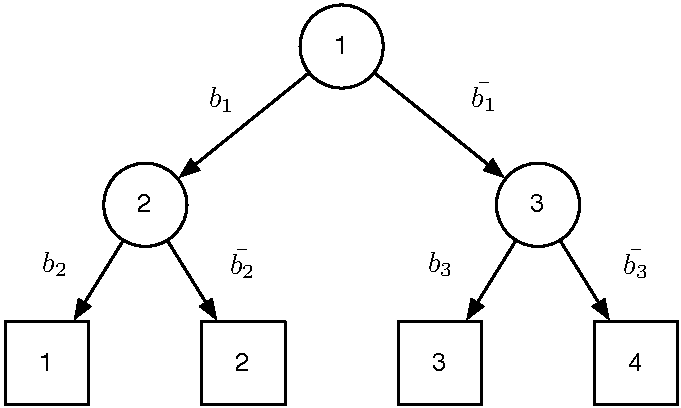
\includegraphics[scale=0.7]{decision_tree.pdf}
	\caption{A decision tree}
	 \label{fig:decision_tree}
\end{figure}

The idea is that the tree is known by the server but has to remain private while the boolean variables are unknown to the server, as well as the associated category.

Let us consider the function $f$ that takes as input the booleans $b_i$ maps them to the category in the decision tree. It is really easy to construct $f$ as multivariate polynomial in the $b_i$s whose degree is the depth of the decision tree (we can construct this polynomial recursively). For example, in the example of figure~\ref{fig:decision_tree}, we have:
\[
	f(b_1,b_2,b_3) = b_1(b_2.1 + (1-b_2).2) + (1-b_1)(b_3.3 + (1-b_3).4)
\]          

We use FHE to evaluate the polynomial over the encrypted $b_i$.
% subsection decision_tree_principle (end)

\subsection{Protocol} % (fold)
\label{sub:decision_tree_protocol}

\subsubsection{Using general FHE} % (fold)
\label{ssub:using_general_fhe}
	In this section, we consider an FHE scheme that is able to compute functions over integers (not only bits).
	
	As input, the server takes the polynomial $f$ corresponding to its decision tree, the public of the FHE scheme, and the encryption of each $b_i$ under this scheme. The server simply evaluates $f$ over these encrypted values using the the FHE scheme's evaluation function. It obtain the encryption of the category's index and sends it to the client (who has the secret key for the scheme).
	
	Security follows from the semantic security of the scheme. 
% subsubsection using_general_fhe (end)                       

\subsubsection{Using FHE over $\F_2$} % (fold)
\label{ssub:using_fhe_over_f_2}
We do not have to assume that we have access to a FHE scheme that can compute over integers: we can compute the result bit by bit using multiple polynomials similar to $f$. E.g. for the previous example, the polynomials over $\F_2$ are 
\begin{align*}
	f_0(b_1,b_2,b_3) &= b_1(b_2.0 + (1-b_2).1) + (1-b_1)(b_3.0 + (1-b_3).1) \\
	f_1(b_1,b_2,b_3) &= b_1(b_2.0 + (1-b_2).0) + (1-b_1)(b_3.1 + (1-b_3).1) \\
\end{align*} 

In this case, we can even use an additional trick: if the scheme supports SIMD slots (as in~\cite{GHS12}), we can evaluate the polynomial
	\[
		\tilde{f}(b_1,b_2,b_3,c_1,c_2,c_3,c_4) =  b_1(b_2.c_1 + (1-b_2).c_2) + (1-b_1)(b_3.c_3 + (1-b_3).c_4)
	\]
for each bit of the result in parallel. The resulting cyphertext will contain the bits of the result, one bit per slot.      

% subsubsection using_fhe_over_f_2 (end)

% subsection decision_tree_protocol (end)

% section decision_trees (end)                                 

\section{Useful protocols} % (fold)
\label{sec:useful_protocols}

For the proofs of security, we show that whatever a party can compute from its view of the protocol can be computed from its input and its output (see Definition 7.2.1 in \cite{Goldreich2}).                                

\subsection{Changing the encryption scheme} % (fold)
\label{sub:changing_encryption_scheme}
	Suppose we have two additively homomorphic encryption schemes $\mathsf{E_1}$ and $\mathsf{E_2}$ with the same message space $M$ and two parties Alice and Bob. Alice has the secret keys $sk_1$ and $sk_2$ for both schemes and Bob has a value encrypted with $\mathsf{E_1}$ with the public keys $pk_1$ and $pk_2$. We propose a protocol that enable Bob to get an encryption of its value under $\mathsf{E_2}$ without revealing anything to Alice. In the following, $*$ represents the homomorphic operation over cyphertexts. 
	
	\begin{itemize}
		\item Alice's input: $(sk_1,sk_2)$; Bob's input: $(pk_1,pk_2,c)$ where $c$ is a cyphertext of $\mathsf{E_1}$ under public key $pk_1$.
		   
		\item Bob picks $r \leftarrow M$ uniformly at random, sets $c' = c * \mathsf{E_1.Enc}(r)$ and sends $c'$ to Alice.
		
		\item Alice decrypts $c'$, re-encrypts the result with the new encryption scheme and sends the new cyphertext $c'' = \mathsf{E_2.Enc}(\mathsf{E_1.Dec}(c'))$ to Bob.
		
		\item Bob outputs $\tilde{c} = c'' * \mathsf{E_2.Enc}(r)$  
		
	\end{itemize}
	      
	\paragraph{Security for Alice} Alice's view is $V_A = (sk_1,sk_2,c')$.\\
	The simulator $S_A$ sends a random encrypted element $c'$ to Alice which is statistically indistinguishable from the real $c'$ (as both are encrypting a value coming from the same uniform distribution over the message space $M$). Thus the tuple $(sk_1,sk_2,c',\tilde{c})$  generated in the ideal setting is indistinguishable from the real setting.

	\paragraph{Security for Bob} Bob's view is $(pk_1,pk_2,c,c'')$.\\   
	We build a simulator $S_B$ (whose inputs are $pk_1$, $pk_2$ and $c$) that produces an encryption $c''$ of a random element. As we suppose $\mathsf{E_2}$ to be semantically secure, Bob's real view and output (the tuple $(pk_1,pk_2,c,c'',\tilde{c})$) is indistinguishable from the simulated view and output.   

% subsection changing_encryption_scheme (end)

\subsection{Comparing encrypted data} % (fold)
\label{sub:comparing_encrypted_data}
	This is a modification of Veugen's work in \cite{Veugen}. 
	
	For the naive Bayes classifier (see \ref{sub:bayes_solution_2}), we want a protocol that obliviously compares encrypted data. Protocol 1 (Client-server comparison) in~\cite{Veugen} is almost what we are looking for, except that A (the party who has the encrypted data without the decryption key) gets an encrypted version of the comparison result. Thus we slightly modify the protocol so that A gets the result in the clear.
	
	In the modified protocol, B no longer has the secret key for the QR (GGM) cryptosystem, A does. So A and B run the LSIC protocol (as defined in~\cite{Veugen}) so that B gets the encrypted bit $[t']$ (encrypting $(d < c)$). Then, we reverse the roles of A and B: 
	\begin{itemize}
		\item A encrypts $r_{l+1}$ and sends $[r_{l+1}]$ to B
		\item B encrypts $z_{l+1}$, computes $[t] \leftarrow [t'].[z_{l+1}].[r_{l+1}]$ and sends $[t]$ to A
		\item A decrypts and outputs $t$
	\end{itemize}
	
	We prove the security of this protocol in the hybrid model where the encrypted bit $[t']$ is ideally computed.
	
	\paragraph{Security for A} A's view is $V_A = (\llb a\rrb,\llb b\rrb,sk_{QR},pk_P,[t])$ where $sk_{QR}$ is the secret key for the QR cryptosystem and $pk_P$ is the public key for Paillier's cryptosystem.\\
	Given $(\llb a\rrb,\llb b\rrb,sk_{QR},pk_P, a \leq b)$, the simulator $S_A$ computes an encryption of the bit $a \leq b$ under QR. The ideal and real executions are the same, then indistinguishable.
	
	\paragraph{Security for B} B's view is $V_B = (pk_{QR}, sk_{P}, \llb z \rrb, [t'], [r_{l+1}])$.\\
	Given $(pk_{QR}, sk_{P})$ as input, the simulator $S_B$ picks a random $\tilde{z} \leftarrow \Z_N$ and generates a Paillier encryption $\llb \tilde{z} \rrb$. $z$ and $\tilde{z}$ are generated according to the same distribution (uniform over $\Z_N$) so $\llb z \rrb$ and $\llb \tilde{z} \rrb$ also are. Finally, $S_B$ encrypts two random bits under QR, $[\tilde{t}']$ and $[\tilde{r}_{l+1}]$. $(pk_{QR}, sk_{P}, \llb z \rrb, [t'], [r_{l+1}])$ is computationally indistinguishable from $(pk_{QR}, sk_{P}, \llb \tilde{z} \rrb, [\tilde{t}'], [\tilde{r}_{l+1}])$ because QR is semantically secure. 
% subsection comparing_encrypted_data (end)

% section useful_protocols (end)


\section{Related Work} % (fold)
\label{sec:related_work}
        
\begin{description}
	\item[Secure Multiparty Computational Geometry] (\emph{Atallah, Du}) Some specialized secure MPC protocol for Computational Geometry. Very interesting for us as one of the problem they solve is point inclusion, which is closely related to hyperplane decision. They give protocols to compute dot products based on 1-out-of-N OT, one of which does not use homomorphic encryption.
	\\ \href{https://www.cerias.purdue.edu/assets/pdf/bibtex_archive/2001-48.pdf}{Link} 
	
	\item [On Private Scalar Product Computation for Privacy-Preserving Data Mining](\emph{Goethals, Laur, Lipmaa, Mielikainen})
	\\ \href{http://eprints.pascal-network.org/archive/00000295/01/sspfordm.pdf}{Link} 
	
	\item [Secure Multiparty Computation of Approximations](\emph{Feigenbaum, Ishai, Malkin, Nissim, Strauss, Wright}) Describes a protocol to efficiently approximate the Hamming distance and \#P-hard functions.                                               
	\\ \href{http://cs-www.cs.yale.edu/homes/jf/FIMNSW.pdf}{Link}
	
	\item [ML Confidential:	Machine Learning on Encrypted Data](\emph{Graepel, Lauter, Naehrig}) An implementation, based on FHE, of basic machine learning classification algorithms.	   
	\\ \href{http://research.microsoft.com/pubs/179548/323.pdf}{Link}
	  
	\item [Privacy-Preserving Support Vector Machines Learning](\emph{Zhan,Chang, Matwin}) How to run a learning algorithm on distributed datas in a private way. They essentially show how to use Paillier to obliviously compute dot products.
	\\ \href{http://iceb.nccu.edu.tw/proceedings/2005/477-482.pdf}{Link}
	                                            
	\item [Cryptographically Private Support Vector Machines](\emph{Laur, Lipmaa,Taneli Mielikainen}) Describes private protocol for ``kernel sharing, prediction and training''. Based on Paillier.
	\\ \href{http://eprint.iacr.org/2006/198.pdf}{Link}
	
	\item [Privacy-Preserving SVM using Nonlinear Kernels on Horizontally Partitioned Data] (\emph{Yu, Jiang, Vaidya})
	\\ \href{http://cimic.rutgers.edu/~jsvaidya/pub-papers/vaidyaSVM-sac06.pdf}{Link}
	      
	\item [Privacy-Preserving SVM Classification on Vertically Partitioned Data] (\emph{Yu, Vaidya, Jiang})
	Check the ``Related Work'' section for a small survey of existing protocols.
	\\ \href{http://link.springer.com/content/pdf/10.1007%2F11731139_74.pdf}{Link}
	
	                                   
	\item [Secure Multiparty Computation Goes Live](\emph{Bogetoft et al.}) A large-scale practical implementation of a secure auction using MPC. They describe and prove lots of efficient cryptographic protocols.  
	\\ \href{http://eprint.iacr.org/2008/068.pdf}{Link}
       
	\item [Unconditionally Secure Constant Round Multi-Party Computation for Equality, Comparison, Bits and Exponentiation](\emph{Damgard, Fitzi, Kiltz, Nielsen, Toft})
	\\ \href{http://www.iacr.org/cryptodb/archive/2006/TCC/3624/3624.pdf}{Link}
             
	\item [Oblivious Polynomial Evaluation](\emph{Naor, Pinkas}) How a receiver can evaluate $P(x)$ where $P$ is a polynomial owned by a sender, without disclosing $x$ while preserving the server's secret ($P$).
	\\ \href{http://citeseerx.ist.psu.edu/viewdoc/download?doi=10.1.1.73.7197&rep=rep1&type=pdf}{Link}
                                                                          
	\item [Efficient Private Matching and Set Intersection](\emph{Freedman, Nissim, Pinkas}) Various secure MPC protocols to compute set intersection of private datasets.
	\\ \href{http://www.cs.princeton.edu/~mfreed/docs/FNP04-pm.pdf}{Link}
	
	\item [Secure Multi-Party Sorting and Applications](\emph{Jonsson, Kreitz, Uddin})
	\\ \href{http://eprint.iacr.org/2011/122.pdf}{Link}
	                  
	\item [State-of-the-art in Privacy Preserving Data Mining](\emph{Verykios, Bertino,Nai Fovino, Parasiliti Provenza, Saygin, Theodoridis})
	\\ \href{http://www.sigmod.org/publications/sigmod-record/0403/B1.bertion-sigmod-record2.pdf}{Link}
	
	\item [An Efficient Solution to The Millionaires' Problem Based on Homomorphic Encryption](\emph{Lin, Tzeng})
	\\ \href{http://eprint.iacr.org/2005/043.pdf}{Link}
	                
	\item [Secure Two Party Comparison over Encrypted Data](\emph{Kaghazgaran, Sadeghyan})
	\\ \href{http://ieeexplore.ieee.org/stamp/stamp.jsp?tp=&arnumber=6141405&tag=1}{Link} 
	
	\item [Practical and Secure Solutions for Integer Comparison](\emph{Gary, Schoenmakers, Villegas})
	Millionaire's protocol for encrypted inputs (the input is given bit by bit).
	\\ \href{http://www.win.tue.nl/~berry/papers/pkc07intcomp.pdf}{Link}   
	
	                                                                                             
	\item [Comparing Encrypted Data](\emph{Veugen}) \cite{Veugen}
 	Millionaire's protocol for encrypted inputs (does not entirely fulfill the requirements we need for the second solution of the Bayes classifier, but may be modified to do so).   
	\\ \href{http://msp.ewi.tudelft.nl/sites/default/files/Comparing%20encrypted%20data.pdf}{Link}
\end{description}


% section related_work (end)



\newpage



\bibliography{main}
\bibliographystyle{alpha}





\end{document}
